\documentclass[12pt]{article}
\usepackage[letterpaper, margin=0.75in]{geometry}
\usepackage{tabularx}
\usepackage{graphicx}
\usepackage{titling}
\usepackage[makeroom]{cancel}
\usepackage{color}

\pretitle{\begin{center}\LARGE
\includegraphics[width=10cm]{../images/logo.png}\\[\bigskipamount]}
\posttitle{\end{center}}

\begin{document}

\begin{center}

\includegraphics[width=10cm]{../images/logo.png}
\end{center}

\begin{center}
\noindent{\LARGE Conceptual Physics \\ Lecture Notes}\footnote{DISCLAIMER: These notes contain typos.}

\vspace{0.1in}
\noindent{Katherine Quinn}
\end{center}

\noindent These lecture notes relate to part two of this course. It is material covered in classes 9 through 13:
\begin{enumerate}
\item Atomic and Particle Theory, and Light
\item Fields of Force
\item Special Relativity
\item General Relativity and Cosmology
\item Quantum Mechanics
\end{enumerate}

\noindent Each part of these notes lists the relevant readings, and then summarizes the relevant material with sample problems.\footnote{DISCLAIMER: The worked examples may also contain typos. I apologize for the vast quantity of typos, but I haven't had time to thoroughly read through the notes and correct every one of them.} Note that while the same material is covered in class 14, the review class, there will be no lecture as that class will be purely reserved for co-op problems and questions.

\section{Atomic and Particle Theory, and Light}

\noindent \textbf{Readings:}
\begin{enumerate}
	\item Chapter 17 (Section 1) of \textit{Light and Matter}
	\item Chapter 19 (Section 3 and 4) of \textit{Light and Matter}
	\item Chapter 26 (Section 1, 4) of \textit{Light and Matter} 
\end{enumerate}

\noindent\textbf{\large The Atomic Model and Particle Theory}
\begin{center}
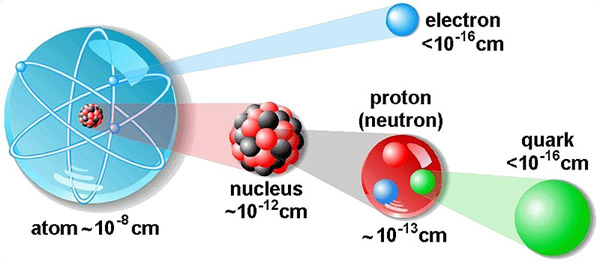
\includegraphics[width=3in]{../images/atoms.jpeg}
\end{center}

\begin{itemize}
	\item Different \textit{elements} have different numbers of \textit{protons}.
	\item Different \textit{isotopes} (of the same element) have different numbers of \textit{neutrons}.
\end{itemize}

The periodic table categorizes all known elements. The sorting is done based on number of protons (left-right, top-down) as well as chemical properties (impacts which elements get put into which column/row).

\begin{center}
\noindent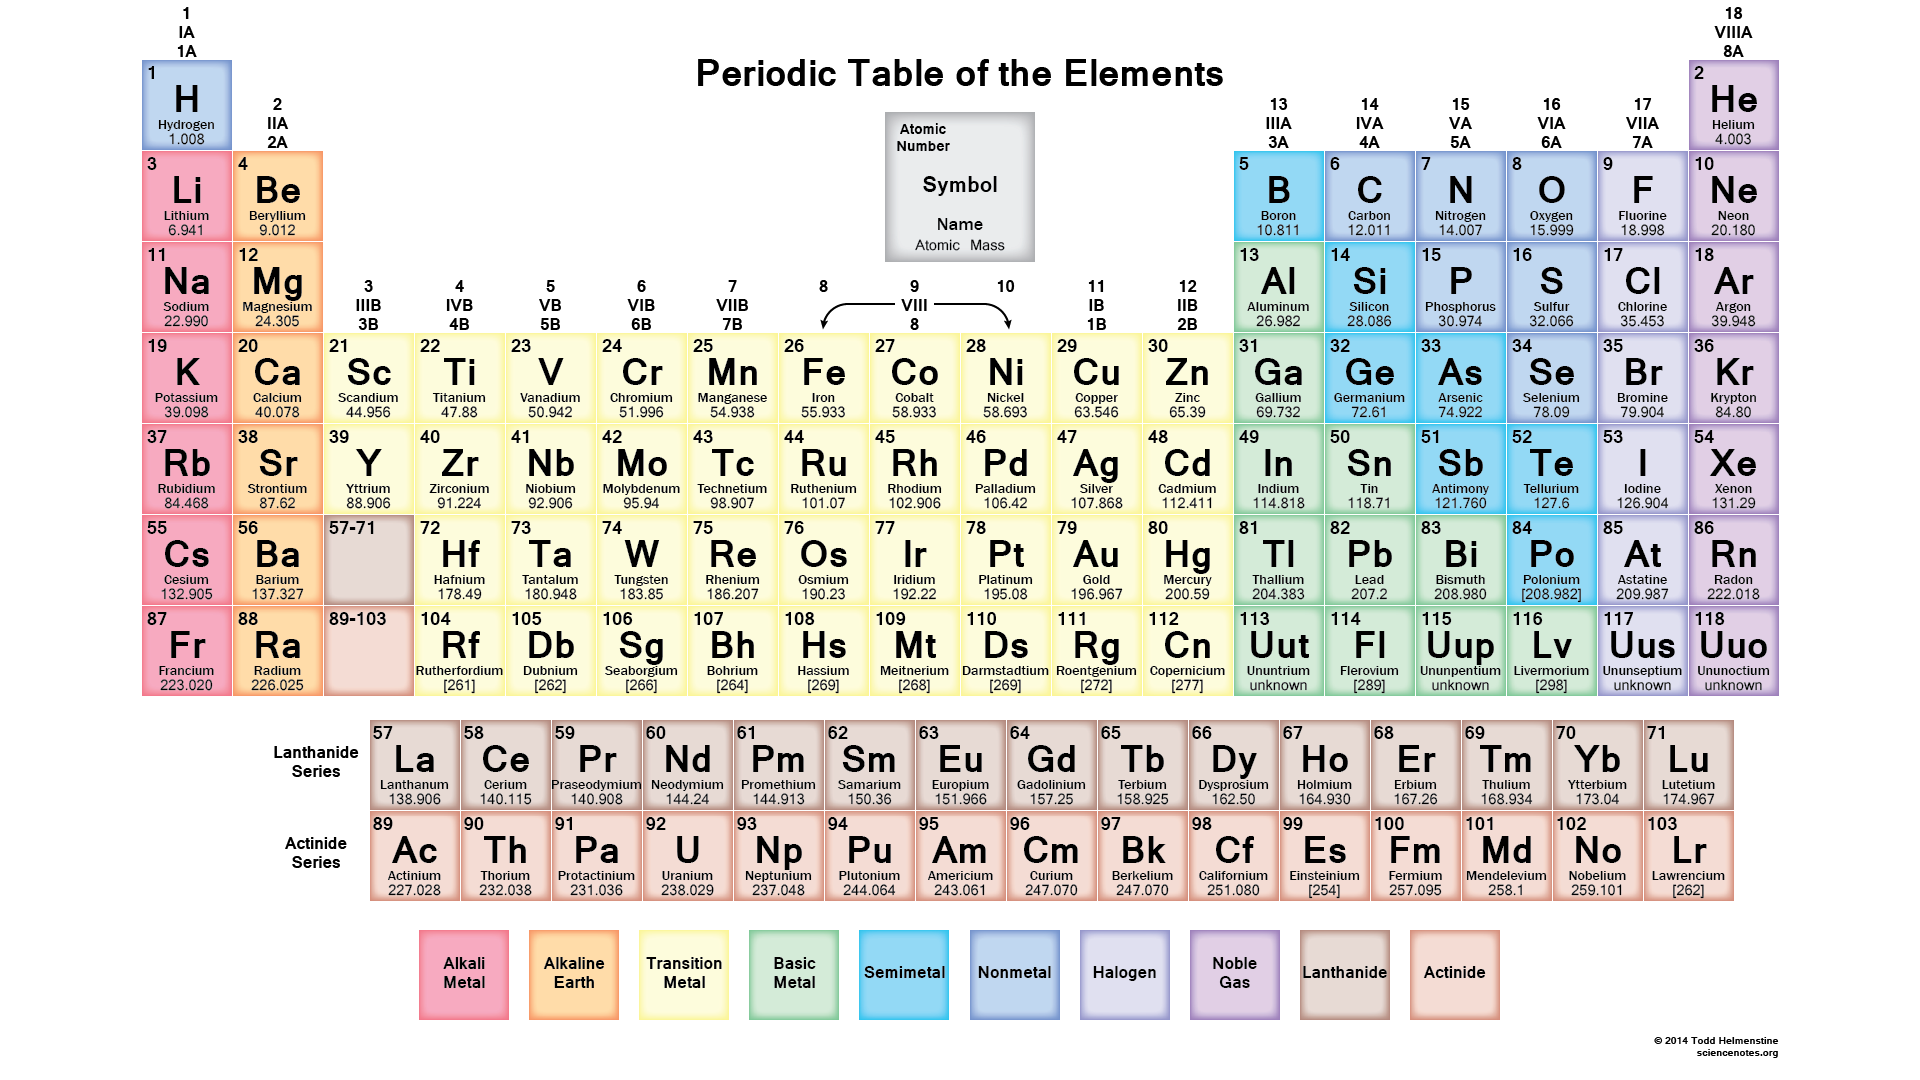
\includegraphics[width=\textwidth]{../images/periodicTable.png}
\end{center}

There are far more known particles than those that make up the elements (electrons, protons, neutrons, quarks). These are divided into \textit{elementary} and \textit{composite} particles:

\begin{itemize}
	\item Elementary particle: Something which cannot be broken down. Some kinds of elementary particles:
	\begin{itemize}
		\item electron (negative charge)
		\item quarks
		\item photons (light particles)
	\end{itemize}
	\item Composite particle: particle composed of elementary particles. Some kinds of composite particles include:
	\begin{itemize}
		\item proton (composed of quarks)
		\item neutron (also composed of quarks)
	\end{itemize}
\end{itemize}

Just like the periodic table sorts all known elements, the fundamental particles can be sorted on a table. These are sorted according to the \textit{Standard Model of Physics}

\begin{center}
	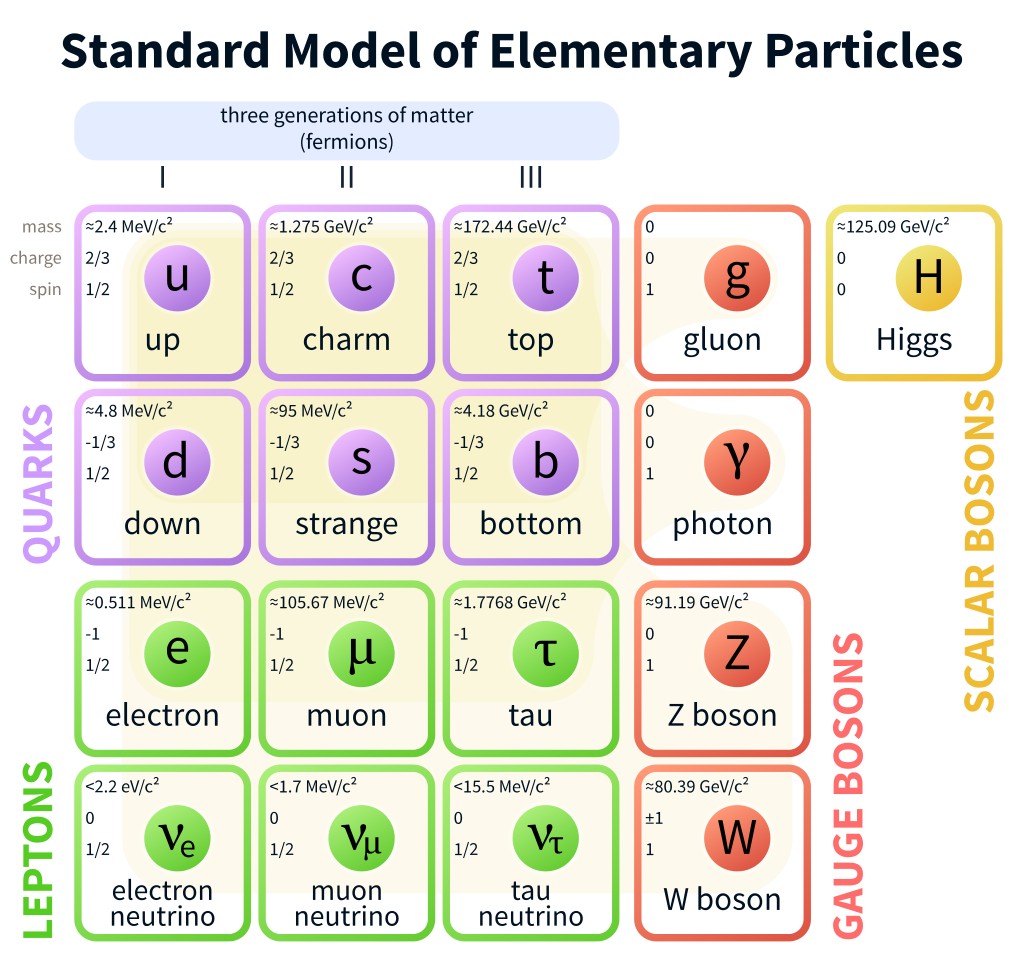
\includegraphics[width=0.5\textwidth]{../images/standard_model.png}
\end{center}

There are a great many composite particles that physicists have detected, beyond just protons and neutrons. In particular, particles that are made up of quarks are called \textit{hadrons.} They tend to be made up of quarks in pairs (called \textit{mesons}) and in triplets (called \textit{baryons}).

\noindent\textbf{\large Light}

Light can be seen as a particle, called the photon. It can also be seen as a wave (composed of electric and magnetic fields): Called an \textit{ElectroMagnetic (EM) Wave}

\begin{center}
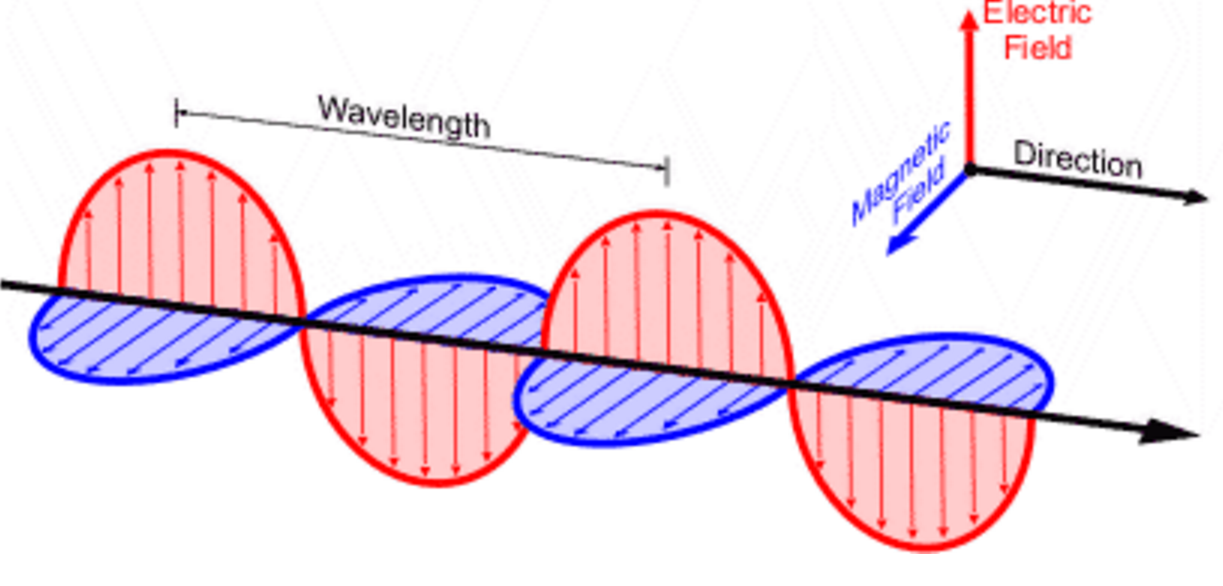
\includegraphics[width=4in]{../images/EMWAVE.png}
\end{center}

In vacuum (without any air or other matter sources in the way) light always travels at the speed of light, which is represented as the letter \textit{c}. This is equal to about $3\times 10^8 m/s$.

Since it is a wave, it is characterized by \textit{wavelength}. This is represented by the Greek letter $\lambda$.

\begin{center}
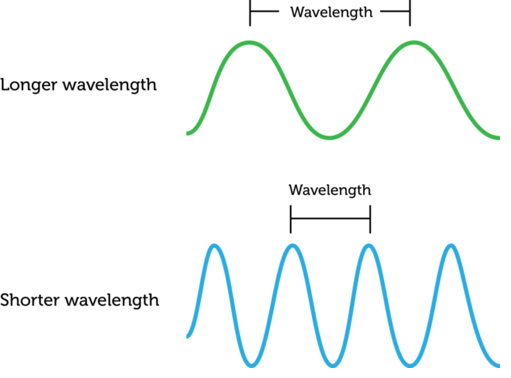
\includegraphics[width=3in]{../images/wavelengths.png}
\end{center}

Light is also characterized by \textit{frequency}, which is like the the inverse of wavelength:
\begin{eqnarray}
f = \frac{c}{\lambda} \nonumber
\end{eqnarray}

The wavelength/frequency of light determines its \textit{energy}. Not all light has the same energy: visible light has much less energy in it than x-rays, for example.

\noindent High energy light:
	\begin{enumerate}
		\item High frequency
		\item Long wavelength
	\end{enumerate}
	
\noindent Low energy light:
	\begin{enumerate}
		\item Low frequency
		\item Short wavelength
	\end{enumerate}

The \textit{electromagnetic spectrum} (EM spectrum) sorts light based on its wavelength/frequency/energy (which are all related)

\begin{center}
\noindent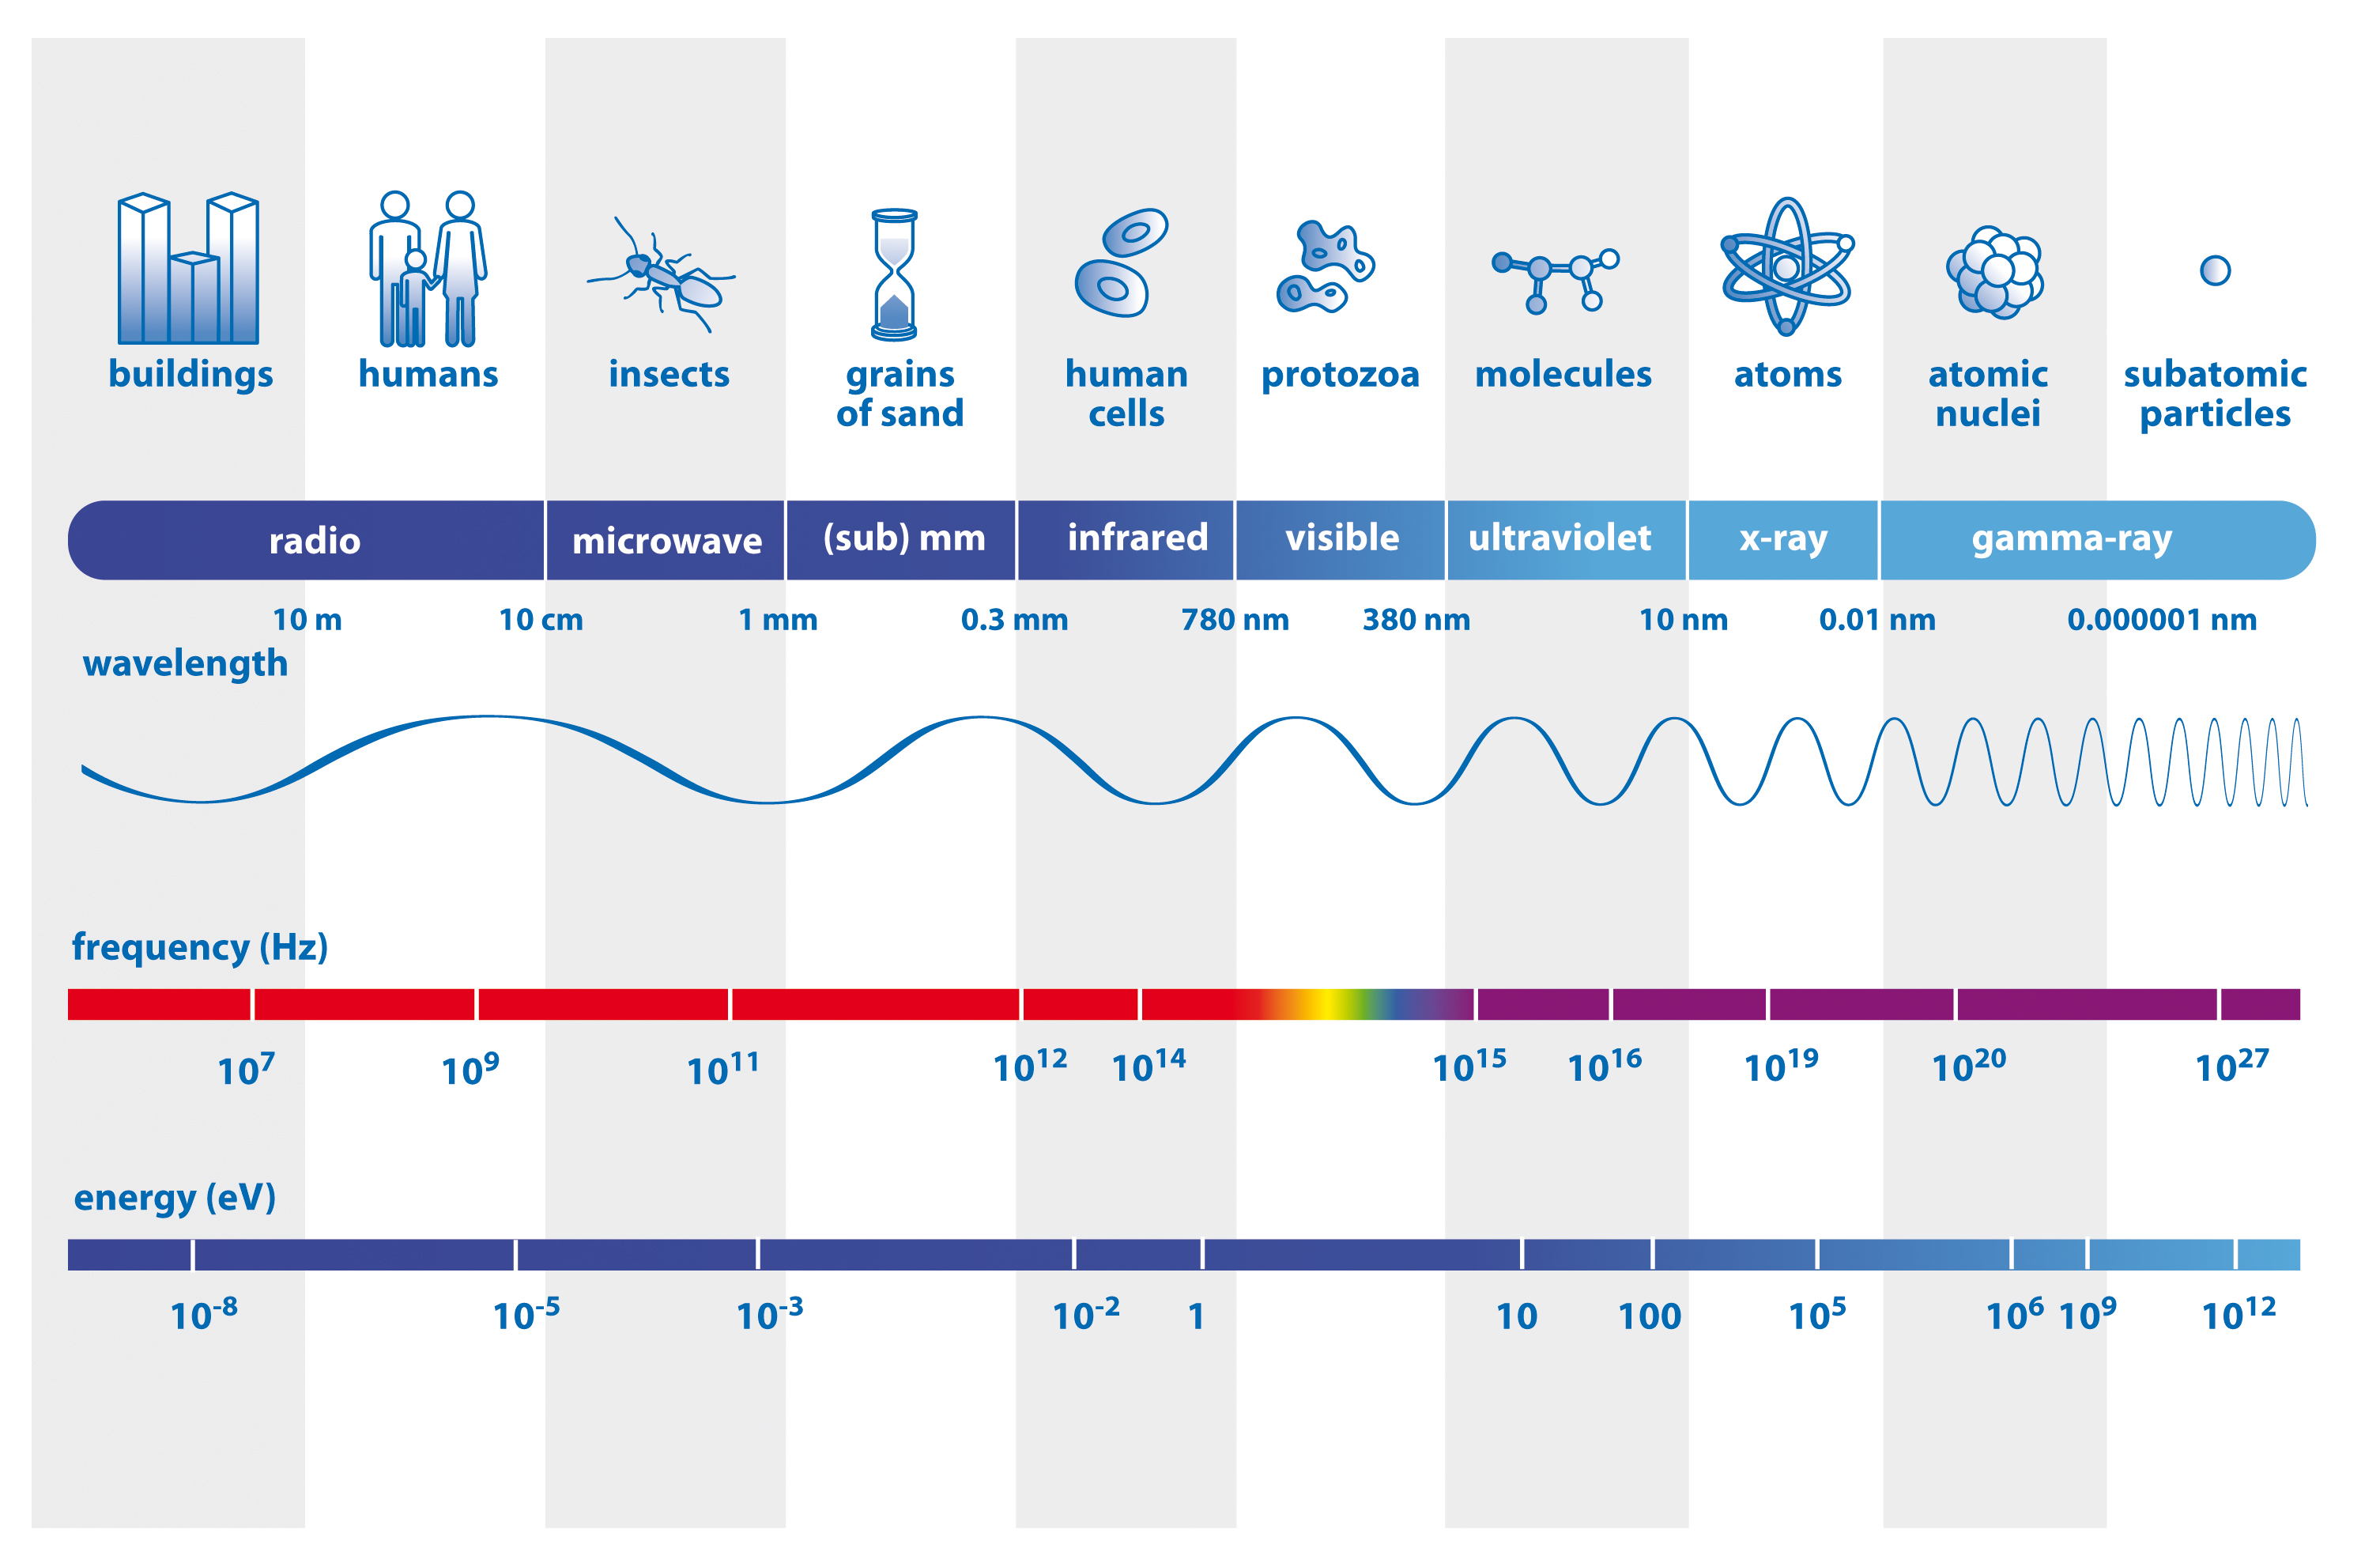
\includegraphics[width=6in]{../images/emSpectrum.jpg}
\end{center}

The frequency and wavelength of light can change. This can happen in 2 ways:
\begin{enumerate}
	\item Blue-Shift: Energy increase (wavelength decrease, frequency increase)
	\item Red-Shift: Energy decrease (wavelength increase, frequency decrease)
\end{enumerate}

Doppler shift: red or blue shift in light, caused by relative motion. The greater the relative velocity, the greater the Doppler shift.
\begin{enumerate}
	\item Source of light and observer are moving together: blue-shifted
	\item Source of light and observer are moving away from each other: red-shifted
\end{enumerate}

\section{Fields of Force}

\noindent \textbf{Readings:}

\begin{enumerate}
	\item Chapter 22 (Sections 1 to 3) of \textit{Light and Matter}
\end{enumerate}

Information cannot travel instantaneously. This means that forces cannot instantaneously effect things at a distance (such as gravity, electric, magnetic, etc.) The fastest information can travel is at the speed of light.

If the Sun disappeared, the Earth would continue to orbit for about 8 minutes. This is because \textbf{actions at a distance have a time delay.} Forces (like gravity), are not transmitted instantaneously; they travel like ``ripples on a pond". Fields of force are a lot like ``traveling force ripples."


     \noindent\begin{tabularx}{\textwidth}{ |X | X }
      \textbf{Electromagnetic and Nuclear Forces} & \textbf{Grativy}
      \\
      -The field represents the carrier particles for these 3 fundamental forces. & -Gravitational fields are the warping of space and time (like a ball on a trampoline). \\
      \raisebox{-\totalheight}{
\includegraphics[width=0.4\textwidth]{../images/carrier.png}}
      & 
      \raisebox{-\totalheight}{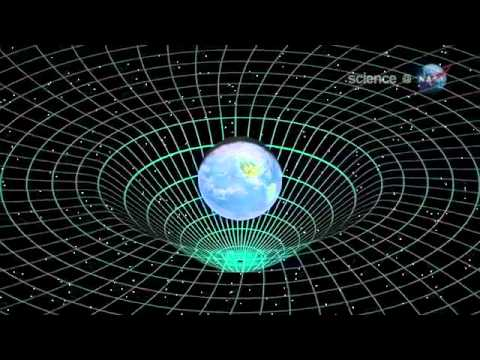
\includegraphics[width=0.45\textwidth]{../images/warpedspacetime.jpg}}
      \\
      \end{tabularx}

\clearpage

We draw fields in 2 different ways, either using a ``Sea of Arrows" or ``Field Lines". For instance, the gravitational field around the Earth can be represented these two ways:

     \noindent\begin{tabularx}{\textwidth}{ |X | X }
      \textbf{Sea of Arrows} & \textbf{Field Lines}
      \\
      \raisebox{-\totalheight}{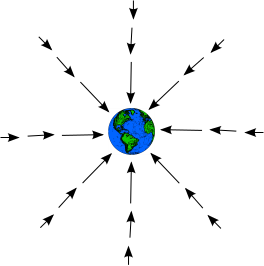
\includegraphics[width=0.45\textwidth]{../images/earthArrows.png}}
      & 
      \raisebox{-\totalheight}{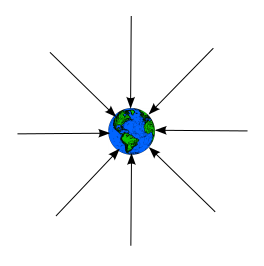
\includegraphics[width=0.45\textwidth]{../images/earthField.png}}
      \\
      -Direction of field is given by direction of the arrow. & -Direction of the field is given by the direction of the arrow. \\
      -Strength of the field is given by the length of the arrow. & -Strength of the field is given by the density of the lines. \\
      -Only 1 arrow at any point in space. & -Field lines can NEVER intersect.
      \end{tabularx}

Fields are defined \textit{operationally}, meaning how to detect/measure them.

\textbf{Gravitational Field}

The gravitational field is the field vector (arrow) at any point in space found by placing a test mass at that point. It is given by
\begin{eqnarray}
g = \frac{F}{m_t} \nonumber
\end{eqnarray}
Where $g$ is the gravitational field (units of $m/s^2$), $F$ is the force on the test mass, and $m_t$ is the size of the test mass.

\textbf{Electric Fields}

\begin{itemize}
	\item Have sources and sinks.
	\item Source: Positive charge
	\item Sink: Negative charge
	\item Electric field lines point in the direction a positive charge would move, and opposite to the direction a negative charge would move.
\end{itemize}

\clearpage

\textbf{Sources and Sinks}

     \noindent\begin{tabularx}{\textwidth}{ |X | X }
      \textbf{Source} & \textbf{Sink}
      \\
      \raisebox{-\totalheight}{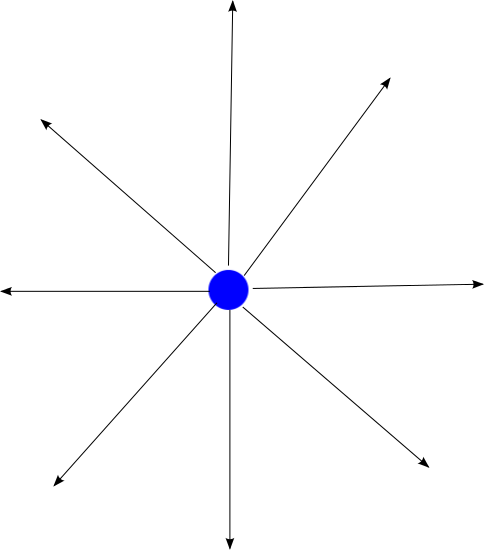
\includegraphics[width=0.45\textwidth]{../images/protonSol.png}}
      & 
      \raisebox{-\totalheight}{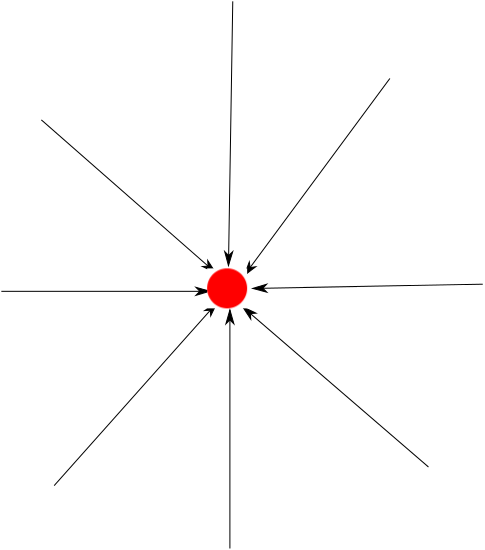
\includegraphics[width=0.45\textwidth]{../images/electronSol.png}}
      \\
      -outward pointing field lines & -inward pointing field lines \\
      \end{tabularx}

Electric field is found by placing a test charge $q$ at a point in space, and looking at the force experienced by that test charge.
\begin{eqnarray}
E = \frac{F}{q} \nonumber
\end{eqnarray}

Here $E$ is the electric field, measured in units of Newtons/Coulomb. 

Similarities with Newton's 2nd Law:
\begin{center}
\input{../images/triangle.pdf_tex}
\end{center}
 
\clearpage
\textbf{Fields with Multiple Sources/Sinks}
Field lines cannot intersect, and they always go from sources to sinks.

     \noindent\begin{tabularx}{\textwidth}{ |X | X }
      \textbf{Examples of Bad Field Lines} & \textbf{Examples of Good Field Lines)}
      \\
      \raisebox{-\totalheight}{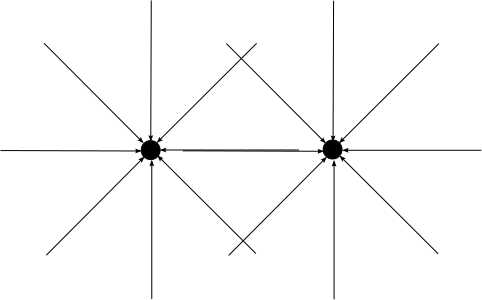
\includegraphics[width=0.45\textwidth]{../images/sinksinkNo.png}}
      & 
      \raisebox{-\totalheight}{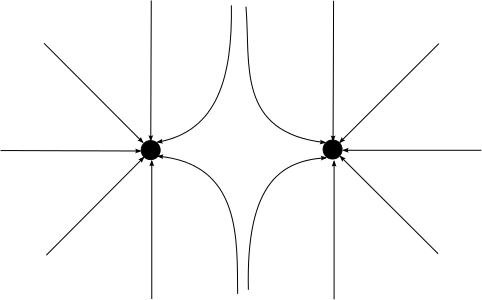
\includegraphics[width=0.45\textwidth]{../images/sinksinkYes.png}}
      \\
      -two sinks & -field lines with crossing field lines ``repel" each other, and bend away \\
      \\
      \raisebox{-\totalheight}{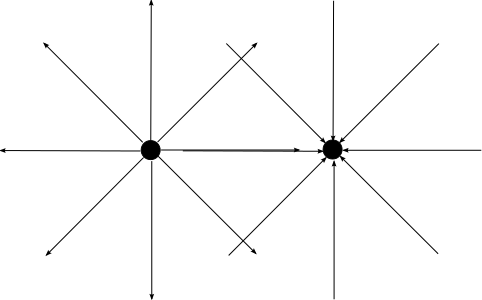
\includegraphics[width=0.45\textwidth]{../images/sinksourceNo.png}}
      & 
      \raisebox{-\totalheight}{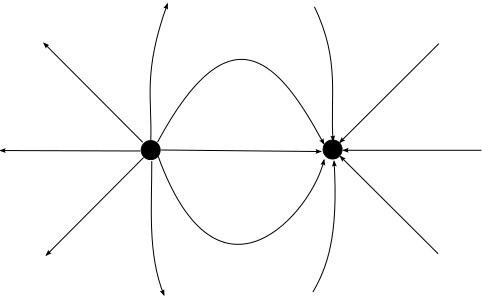
\includegraphics[width=0.45\textwidth]{../images/sinksourceYes.png}}
      \\
      -a sink and a source with crossing field lines & -field lines ``join together", creating a dipole \\
      \end{tabularx}

Gravity: Has only sinks

Electric Force: Has both sources and sinks.
\vspace{0.2in}

\textbf{Force Vs. Field of Force}

     \noindent\begin{tabularx}{\textwidth}{ |X | X }
      \textbf{Force} & \textbf{Field of Force} \\
      -Def: Interaction between 2 objects, causing a push or a pull & -Def: Defined operationally, using a force on a test mass/charge \\
      -Need 2 objects & -Exists throughout all space, with 1, 2, 3, ... objects.
      \end{tabularx}

\clearpage

\section{Special Relativity}

\noindent \textbf{Readings:}

\begin{enumerate}
	\item Chapter 23 (Section 1) of \textit{Light and Matter}
	\item Chapter 28 (Sections 1, 2, 3) of \textit{College Physics}
\end{enumerate}

There is no ``ultimate" frame of reference: All reference frames are equally valid. However, different frames of reference can yield different observations, but they are all ``correct" since none of them are preferred/ultimate.

Space and time are not completely separate, but come together to form \textit{spacetime} (a 4-dimensional continuum).

Some definitions:
\begin{enumerate}
	\item \textit{Special relativity:} The study of how different observers measure the same event.
	\item \textit{Causality:} When one event caused another event. All reference frames agree on causality.
	\item \textit{Simultaneity:} Events occur at the same time. \textit{Not} all reference frames agree on simultaneity.
\end{enumerate}

There are 2 kinds of reference frames:
\begin{enumerate}
	\item \textbf{Inertial:} Non-accelerating reference frame (objects do not accelerate with no cause).
	\item \textbf{Non-Inertial:} Accelerating reference frame, or a frame in a gravitational field. (objects can accelerate with no apparent cause). An example of this would be on the surface of the Earth, or in a rotating/spinning reference frame.
\end{enumerate}

This means there are 2 kinds of relativity:
	\begin{enumerate}
		\item \textbf{Special Relativity:} Observers moving at a constant velocity (in an inertial reference frame)
		\item \textbf{General Relativity:} Observers are in a non-inertial reference frame (accelerating or in a gravitational field.)
	\end{enumerate}

Einstein's postulates:
\begin{enumerate}
	\item Laws of physics are the same in all inertial reference frames.
	\item Speed of light $c$ is the same in all inertial reference frames.
\end{enumerate}

\textbf{Space and Time Distortions}
\begin{itemize}
	\item Time dilation: Time passes slower for an observer moving with respect to another observer, or in a stronger gravitational field than/accelerating with respect to another observer
	\item Length contraction: Shortening of the measured length of an object relative to the observer's frame along the direction of relative velocity.
\end{itemize}

The greater the relative motion, the the greater the effect of time dilation/length contraction. 
\begin{itemize}
	\item Proper time: The time between two events, measured in a reference frame in which the two events occur in the same location (shortest possible measured time).
	\item Proper length: The length of an object measured in its own reference frame, i.e. a frame not moving with respect to the object (longest possible measured length)
\end{itemize}

\textbf{Simultaneity}

Different observers in different reference frames moving with respect to each other do not agree on whether or not events occur simultaneously

(Ex: Light and matter, chapter 23) The garage paradox. Suppose we take a schoolbus and drive it at relativistic speeds
into a garage of ordinary size, in which it normally would not fit.
Because of the length contraction, it fits. But the driver will per-
ceive the garage as being contracted and thus even less able to
contain the bus.
\begin{center}
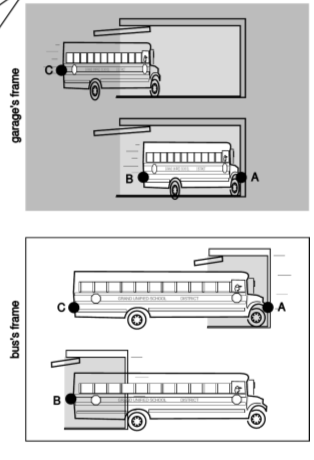
\includegraphics[width=2in]{../images/buses.png}
\end{center}
The paradox is resolved when we recognize that the concept of
fitting the bus in the garage “all at once” contains a hidden as-
sumption, the assumption that it makes sense to ask whether the
front and back of the bus can simultaneously be in the garage.
Observers in different frames of reference moving at high rela-
tive speeds do not necessarily agree on whether things happen
simultaneously. As shown in figure v, the person in the garage’s
frame can shut the door at an instant B he perceives to be si-
multaneous with the front bumper’s arrival A at the back wall of
the garage, but the driver would not agree about the simultaneity
of these two events, and would perceive the door as having shut
long after she plowed through the back wall.

\clearpage

\section{General Relativity}

\noindent\textbf{Readings:}
\begin{enumerate}
	\item Chapter 27 of \textit{Light and Matter}
\end{enumerate}

Spacetime is distorted by mass/energy, and the motion of mass/energy is determined by the bending of spacetime.

     \noindent\begin{tabularx}{\textwidth}{ |X | X }
      \textbf{Flat Spacetime} & \textbf{Real Spacetime} \\
      \raisebox{-\totalheight}{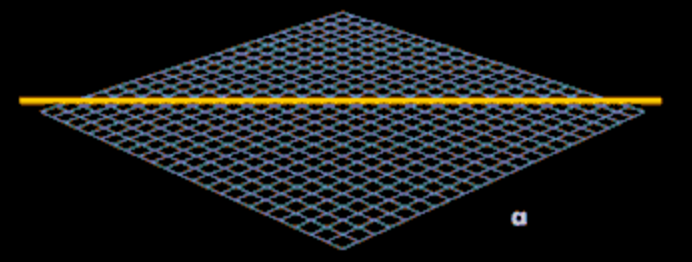
\includegraphics[width=0.45\textwidth]{../images/euclidean.png}}
      & 
      \raisebox{-\totalheight}{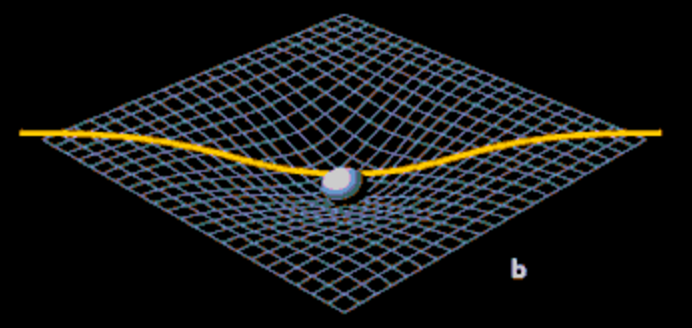
\includegraphics[width=0.45\textwidth]{../images/realSpaceTime.png}}
      \\
      Flat spacetime looks like a rigid grid. & Anything with mass/energy warps and distorts spacetime. \\
      \end{tabularx}
The effects of warped spacetime include:
\begin{enumerate}
	\item Light not does travel in a straight line, it bends and warps around objects. (This contradicts the Newtonian model of the universe, in which light travels in a straight line. We are able to observe the effect of light bending around objects, and this is in fact used to disprove Newtonian model).
	\item Light is red/blue shifted as it falls into/out of gravitational wells.
\end{enumerate}

\textbf{Black Hole:} When an object is so dense that it warps spacetime so much that even light cannot escape its gravitational well. The path of light is so bent that it cannot come out the other side.

\textbf{Gravitational Lensing:} Light bends around large gravitational wells (such as those caused by galaxies and black holes).


     \noindent\begin{tabularx}{\textwidth}{ |X | X }
      \textbf{Model of Gravitational Lensing} & \textbf{Image From Hubble Telescope Showing Gravitational Lensing (of a blue galaxy that is behind a red one)} \\
      \raisebox{-\totalheight}{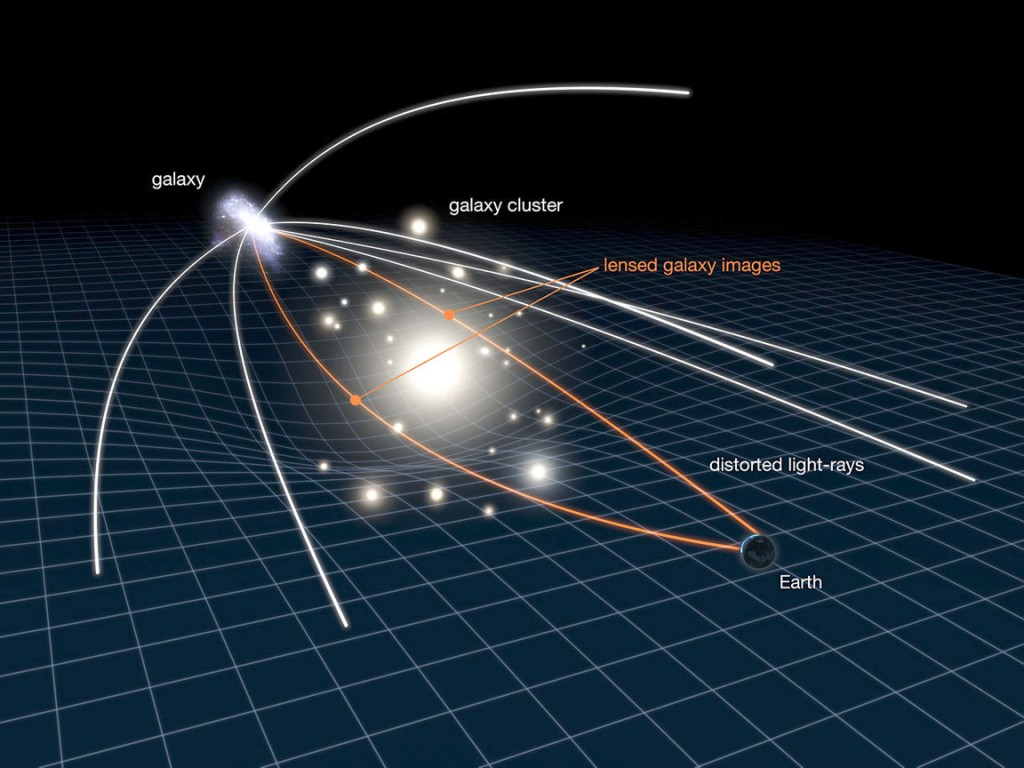
\includegraphics[width=0.45\textwidth]{../images/gravLensingModel.jpg}}
      & 
      \raisebox{-\totalheight}{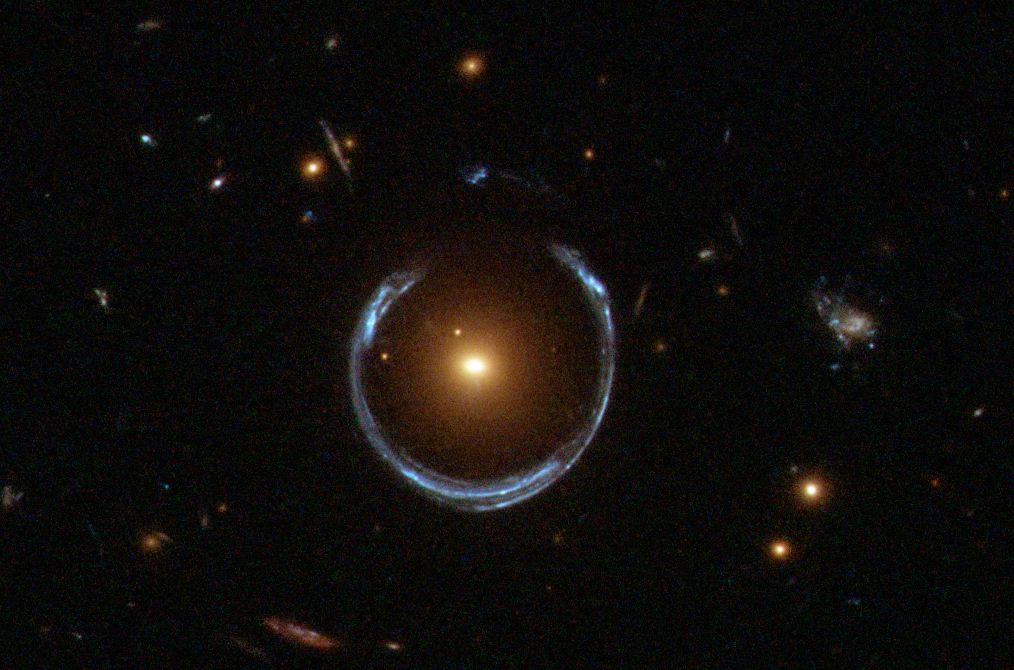
\includegraphics[width=0.45\textwidth]{../images/hubbleLens.JPG}}
      \\
      \end{tabularx}

\clearpage

\textbf{Gravitational waves:} Ripples in spacetime that can travel like waves.
\begin{center}
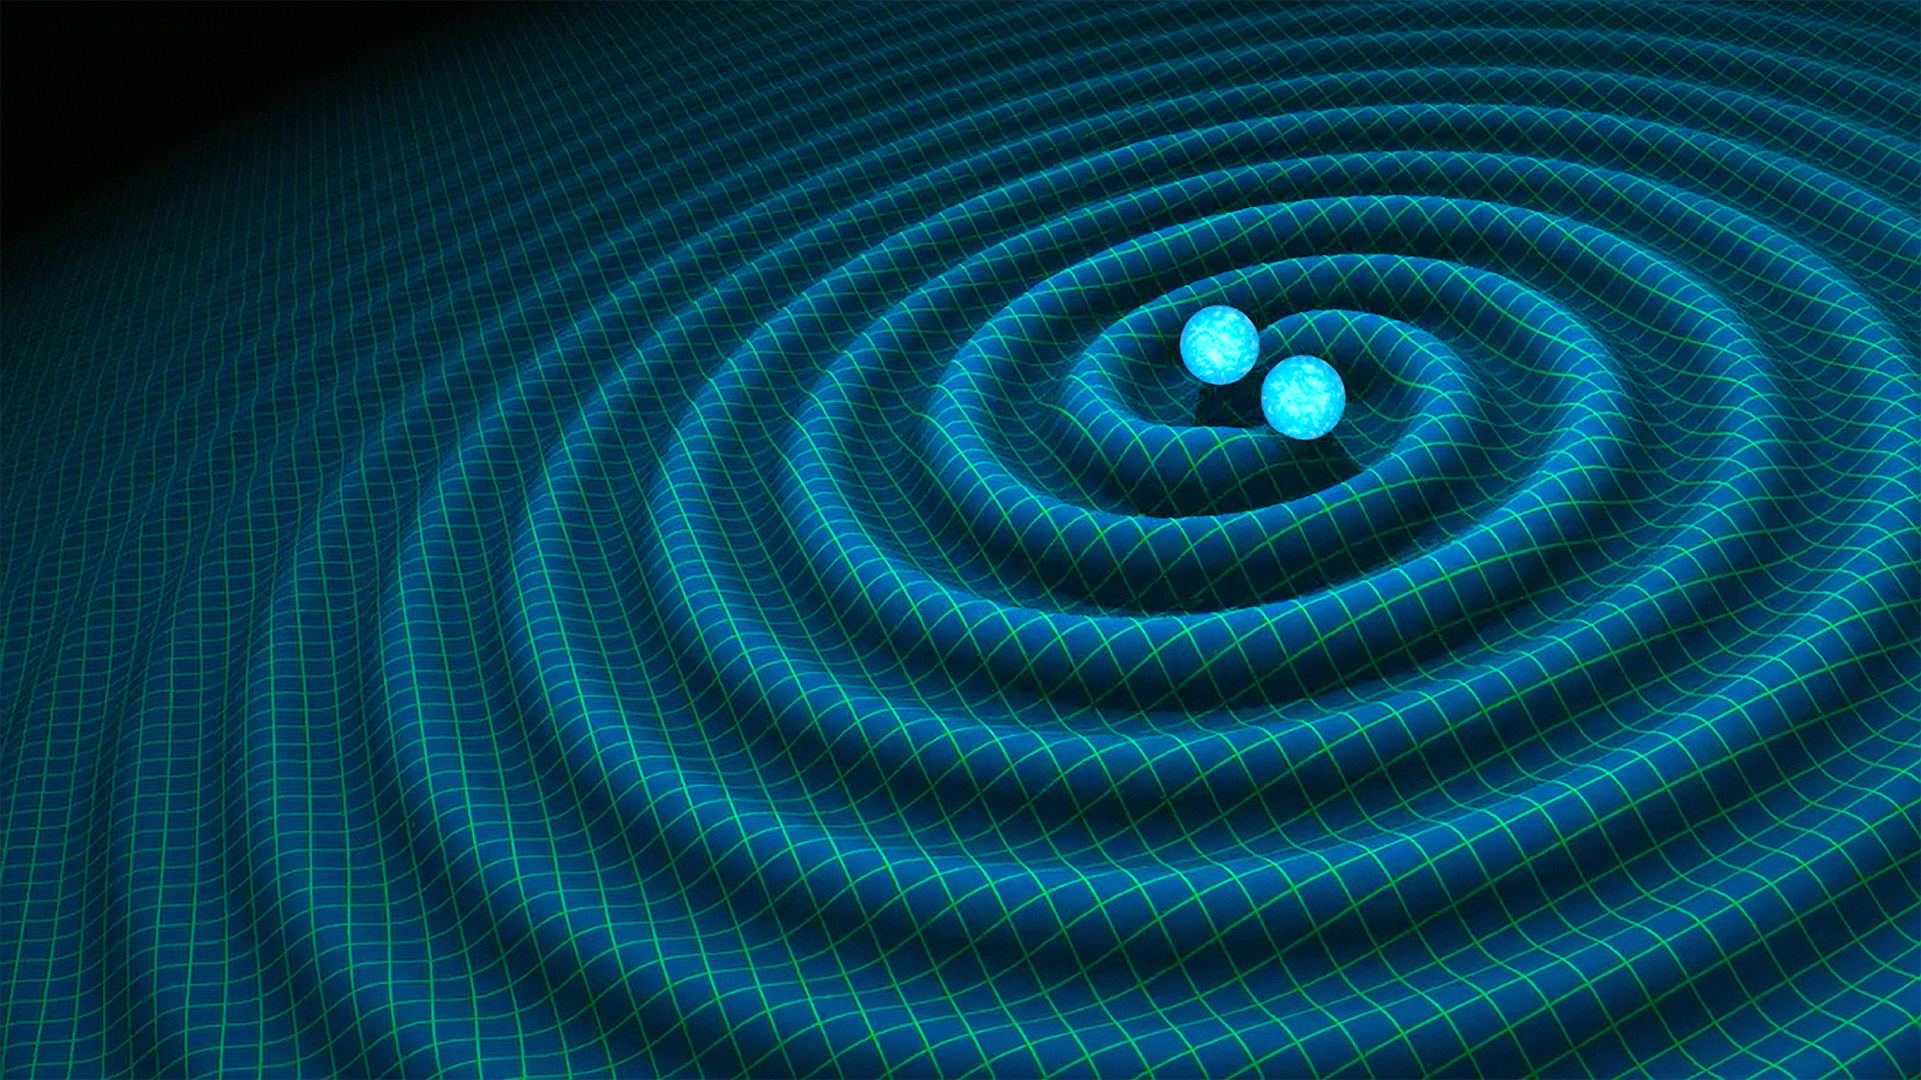
\includegraphics[width=3in]{../images/ligo.jpg}
\end{center}

LIGO: laser interfereometer gravitational-wave observatory detected these from 2 colliding black holes.

Gravitational waves cause minor distortions in spacetime, that cause certain directions to be stretched and others to shrink.

\textbf{Equivalence Principle}

Acceleration is equivalent to a gravitational field, and no observer can tell the difference without an external reference. When an object is in \textit{free fall}, it does not experience gravity.

Gravitational Doppler Shifts are created as light travels in a gravitational field.
	\begin{itemize}
		\item As light falls into a gravitational field, it is blue-shifted.
		\item As light escapes from a gravitational well, it is red-shifted.
	\end{itemize}
	
There are 2 ways to explain the gravitational Doppler shift, using an example of a redshift:
	\begin{enumerate}
		\item \textbf{Equivalence Principle:} Light travelling out of a gravitational well is the same as light travelling in an accelerating elevator. If the light is emitted at the bottom of the elevator, then reaches the top, the relative velocity between the top and the bottom of the elevator is such that they appear to be moving apart (the elevator accelerates in the time it takes the light to travel). Light would therefore appear red-shifted.
		\item \textbf{Energy:} As light move out of a gravitational well, it gains gravitational potential energy. Since energy must be conserved, this causes the energy of the light itself to decrease, causing a red-shift.
	\end{enumerate}

\textbf{Gravitational Time Dilation}

For 2 observers, time is dilated for the observer in the stronger gravitational field. This has been experimentally tested by looking at 2 atomic clocks, one at see level and another high on a mountain (further away from the center of the Earth, and therefore in a smaller gravitational field). The two were ticking at different rates. 

By the equivalence principle, this means time is also dilated for the observer experiencing the greater acceleration.

\vspace{0.3in}
\noindent\textbf{\large Cosmology}

Observation: Most galaxies appear red-shifted, meaning they are moving away from us. Furthermore, the further out we look, the more red-shifted things appear to be: therefore things are moving apart faster, the further apart they are.

Everything appears to be moving away from everything else (with small local exceptions, such as stars within our galaxy). The further back in time you go, things would appear to be closer together; The Big Bang. Illustration: Expanding balloon. As time increases, the distance between galaxies increases (although the size of the galaxies themselves remains the same).
\begin{center}
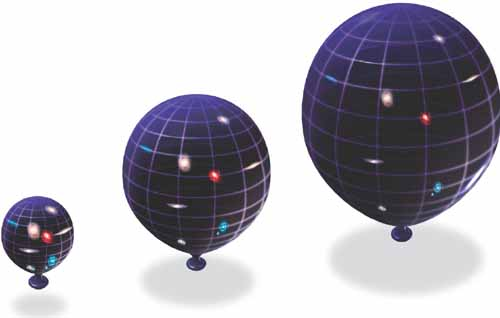
\includegraphics[width=3in]{../images/balloonUniverse.jpg}
\end{center}


This observation is a major contributor to our modern cosmological model;

\noindent\begin{center}
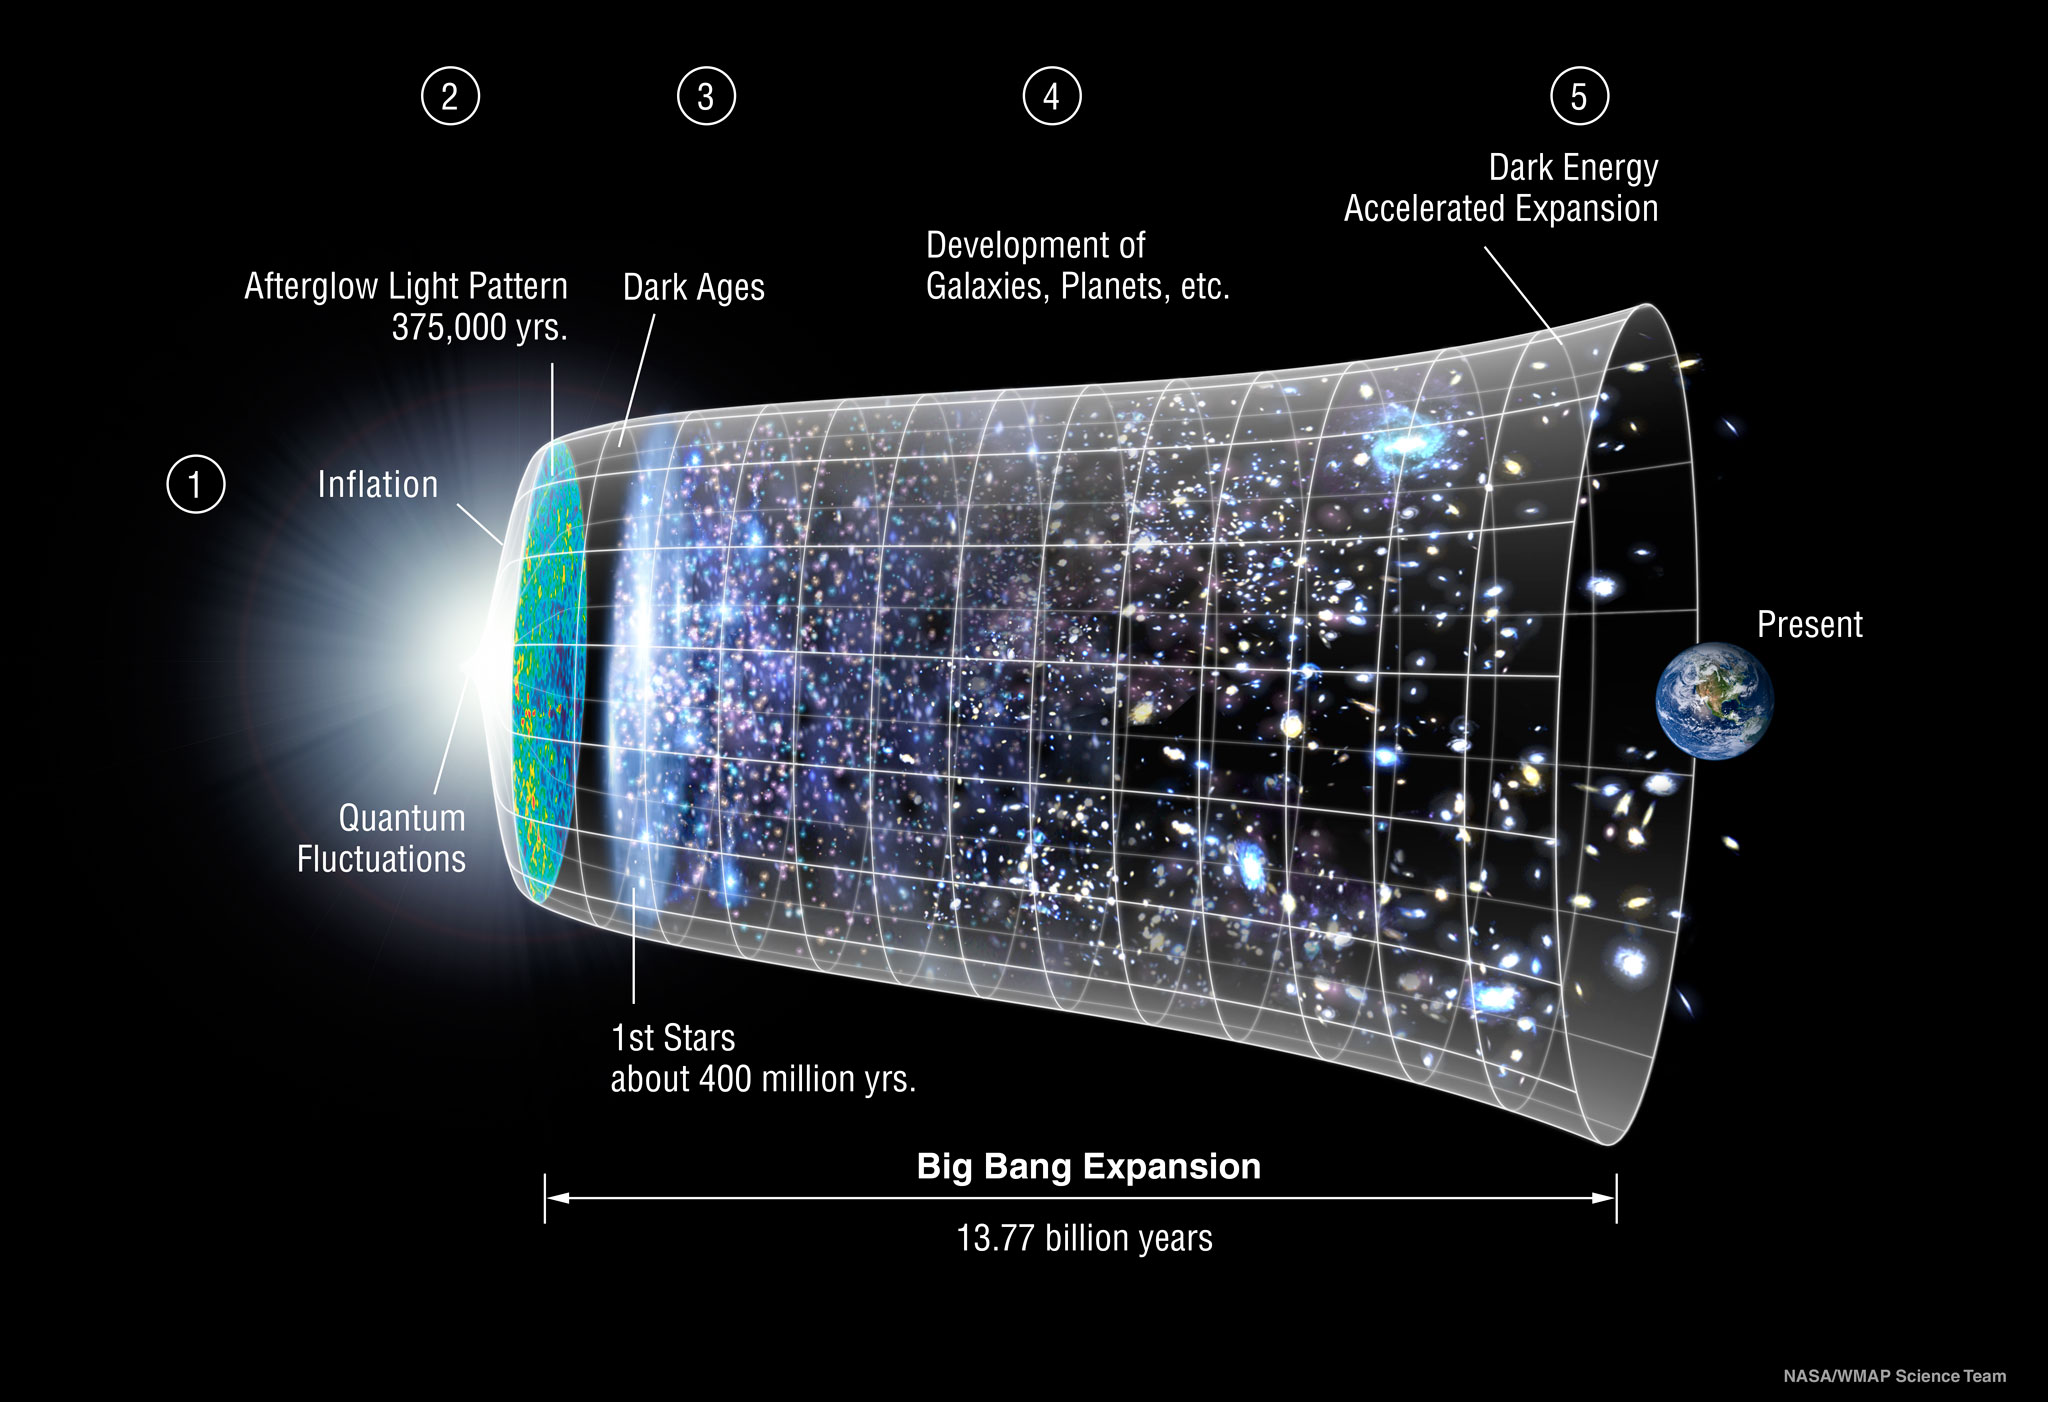
\includegraphics[width=5in]{../images/universeTimeLine.jpg}
\end{center}

\begin{enumerate}
	\item \textbf{Inflation: }A period of rapid expansion, after the big bang.
	\item \textbf{Afterglow:} The universe cooled to the point that light and matter decoupled from each other, resulting in primordial light that we can still detect today. It is known as the cosmic microwave background, and is heavily studied since it is our best probe of the early universe.
	\item \textbf{Dark Ages: }A period of darkness in the universe, as stars hadn't yet formed and so there was no starlight.
	\item \textbf{Development of Galaxies:} Matter began clustering together to form galaxies, composed of billions and billions of stars each.
	\item \textbf{Accelerated Expansion:} Our current period, where the universe has begun a period of accelerated expansion. No one knows why this is happening.
\end{enumerate}

\clearpage

\section{Probability}

\noindent\textbf{Readings:}
\begin{enumerate}
	\item Chapter 33 (Sections 1, 2, 4) of \textit{Light and Matter}
	\item Chapter 34 (Section 1 to 3) of \textit{Light and Matter}
	\item Chapter 35 (Section 1) of \textit{Light and Matter}
\end{enumerate}

\textbf{Determinism:} All events are predetermined. If you knew all forces, and the location and velocity of all objects, you would know everything about the past, present and future.

This is \textit{not} true at atomic scales: Things are described probabilistically.

\vspace{0.1in}
\textbf{Describing Probability}

\begin{itemize}
	\item Impossible event: p = 0 (0\% chance)
	\item Guaranteed event: p = 1 (100\% chance)
	\item 1/2 odds: p = 0.5 (50\% chance)
	\item 1/4 odds: p = 0.25 (25\% chance)
\end{itemize}

\textbf{Statistically independent events:} The odds of 1 event happening do not impact the odds of another event happening. Ex: successive coin flips.

There are different ways of combining probabilities:

\begin{enumerate}
	\item To find the probability of 2 independent events happening, their probabilities are multiplied: If $P_A$ and $P_B$ are the probabilities of 2 statistically independent events, then the likelihood that both A and B will happen is given by $P_A \times P_B$.
	\item To find the probability of either A \textit{or} B happening, their probabilities are added together. If $P_A$ and $P_B$ are the probabilities of 2 events, then the likelihood that A or B will happen is given by $P_A + P_B$.
\end{enumerate}

Ex: Rolling 2 dice. The odds of both being 6 is $1/6\times 1/6 = 1/36$. When rolling 1 dice, the odds of rolling a 5 or a 6 is given by $1/6 + 1/6  = 1/3$.

\textbf{Normalization}: The idea that probabilities for something with multiple possible outcomes must all add up to 1 (there is a 100\% chance that something will happen).
Ex: Rolling dice. The odds that a 1,2,3,4,5 or 6 will be rolled is $1/6+1/6+1/6+1/6+1/6+1/6 = 1$.

\textbf{Averages}: Fro $N$ independent events, each with a probability $P$ of happening, it will happen on average $N\times P$ times.

Example: you have a 1/6 chance of rolling a 5, and so if you were to roll 42 dice you would expect about $42\times 1/6 = 7$ of them to be a 5.

\clearpage

\noindent\textbf{\large Radioactive Decay}

Radioactive decay is the breakdown of an atomic nucleus, resulting in the release of matter and/or energy. There are several kinds of radioactive decay. The 3 main ones are:

\begin{table}[h!]
     \begin{center}
     \begin{tabularx}{\textwidth}{ |X | X | X}
      \textbf{Alpha Decay} & \textbf{Beta Decay} & \textbf{Gamma Decay}\\
      \raisebox{-\totalheight}{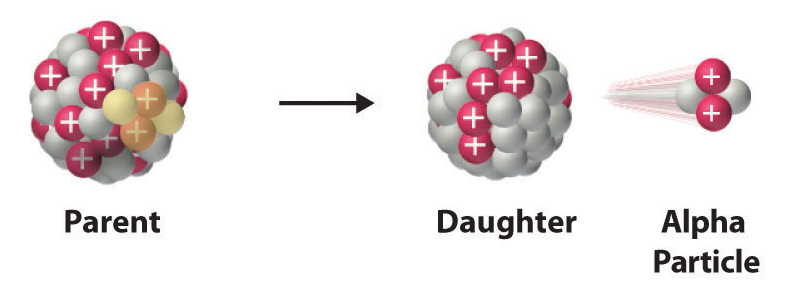
\includegraphics[width=0.3\textwidth]{../images/alpha.png}}
      & 
      \raisebox{-\totalheight}{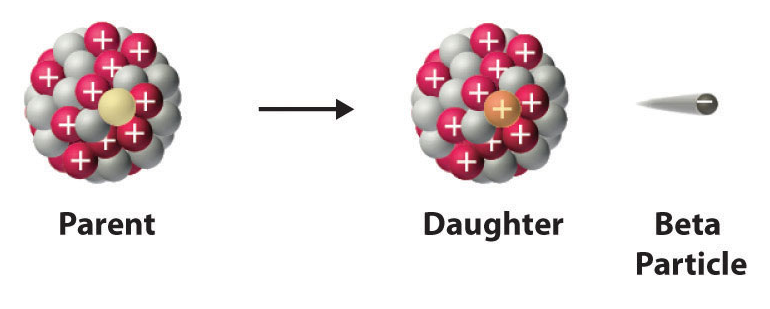
\includegraphics[width=0.3\textwidth]{../images/beta.png}}
      & 
      \raisebox{-\totalheight}{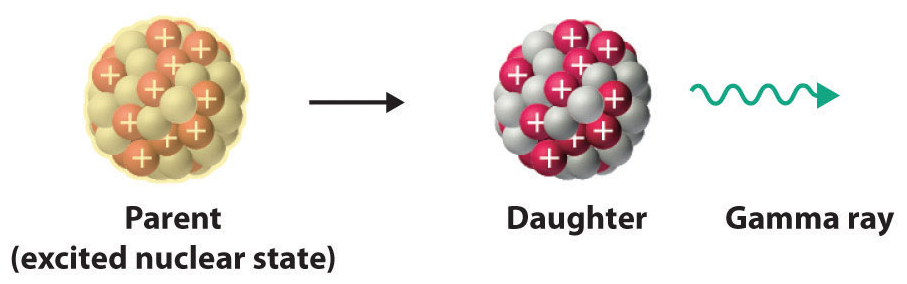
\includegraphics[width=0.3\textwidth]{../images/gamma.png}}
      \\
      Emits an alpha particle (2 protons and a neutron) & Neutron turns into a proton, and emits a beta particle (electron) & A complicated kind of nuclear decay, where an excited nucleus has a lot of extra energy and relaxes, releasing the energy in the form of a gamma ray (light/radiation)
      \end{tabularx}
      \end{center}
\end{table}

\textbf{Describing Radioactive Decay}
\begin{itemize}
\item Described probabilistically.
\item half-life: time at which the probability of an atom to decay is 50\%. (in other words, the time at which you expect 1/2 of a collection of radioactive atoms to decay)
\item half-life depends on the element (and isotope)
\end{itemize}

Useful for dating objects. Ex: Carbon Dating (from Light and Matter, chapter 33)
\begin{center}
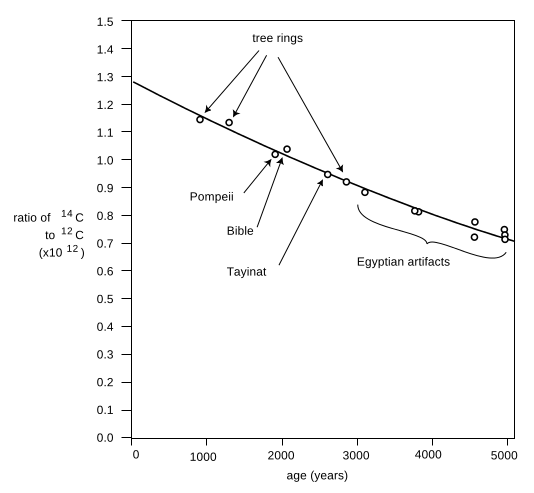
\includegraphics[width=4in]{../images/carbonDating.png}
\end{center}

Almost all the carbon on Earth is C, but not quite. The isotope
$~^{14}$C, with a half-life of 5600 years, is produced by cosmic rays in
the atmosphere. It decays naturally, but is replenished at such a
rate that the fraction of $~^{14}$C in the atmosphere remains constant,
at $1.3\times 10^{-12}$. Living plants and animals take in both $~^{12}$C and
$~^{14}$C from the atmosphere and incorporate both into their bodies.
Once the living organism dies, it no longer takes in C atoms from
the atmosphere, and the proportion of $~^{14}$C gradually falls off as
it undergoes radioactive decay. This effect can be used to find
the age of dead organisms, or human artifacts made from plants
or animals. Figure j shows the exponential decay curve of 14 C
in various objects. Similar methods, using longer-lived isotopes,
prove the earth was billions of years old, not a few thousand as
some had claimed on religious grounds.

\textbf{Wave-Particle Duality}: Light and matter can exist as both particles and waves.

\textbf{Electrons}

Electrons have mass, and can impact objects. We normally think of electrons as particles. They can, however, also be seen as waves. They show the same interference pattern as light, when passing through slits.

\textbf{Wavelength of Matter}

Wavelength is based on energy and momentum (or, equivalently, on mass and velocity).
\begin{itemize}
	\item The more energy something has, the shorter its wavelength.
	\item The more momentum something has, the shorter its wavelength.
	\item The bigger/more massive something is, the shorter the wavelength
	\item The faster something is moving, the shorter the wavelength.
\end{itemize}

Correspondence principle: On large scales for small velocities, quantum effects are not noticeable and thus physics can be described classically.

\textbf{Quantization}

\begin{itemize}
	\item Energy (and momentum) is quantized; comes in discrete packets.
	\item Units of quantization is Planck's constant, h or $\hbar$.
\end{itemize}

\textbf{Photoelectric Effect:} When a photon (light) strikes the surface of an object it can knock out an electron. This can be detected in metals, for instance by shining a light on a circuit and observing a current. It occurs because:
\begin{itemize}
	\item Photons contain energy.
	\item When electrons in an atom absorb photons, they gain the photon's energy. This allows them to gain enough electrical potential energy to ``escape" the atom.
	\item There is a minimum amount of energy needed for an electron to be ejected. If a photon has less energy than this, it is not absorbed an no current is detected. If a photon has greater energy than this, the electron is escapes the atom and the extra energy is converted to kinetic energy.
\end{itemize}

\textbf{Heisenberg Uncertainty Principle}: It is not possible, even in principle, to know the momentum and position of a particle simultaneously with perfect accuracy.

Example: An electron in a box. As the box is made smaller, we better know its position but its bouncing makes it harder to determine it's velocity/momentum.

\textbf{Superposition of States}

Atoms can simultaneously exist in 2 different states. An example of this is in computing, where a bit is described as a 1 or a 0. A quantum-bit (qubit) can exist as \textit{both} a 0 and a 1, in a superposition of states. This idea is driving many physicists to come up with quantum computers, which try to use this effect to facilitate computations.

Similar idea for Shr{\"o}diner's cat: it can be simultaneously dead and alive.


\end{document}